\documentclass[oneside,a4paper,14pt]{extarticle} %размер шрифта 14
\usepackage[T1,T2A]{fontenc}
\usepackage[
	a4paper,
	letterpaper,
	top=2cm,
	bottom=2cm,
	left=2.5cm,
	right=1.5cm
]{geometry}
\usepackage[utf8]{inputenc} %кодировка текста
\usepackage[russian]{babel} %поддержка русского языка
\usepackage{textcomp} %текстовые символы
\usepackage{indentfirst} %корректировка отступов
\usepackage{listings} %для кода !!
\usepackage{float} % для "впихивания" изображений в странницу
\usepackage{xcolor}
\usepackage{enumitem} %для нумерации буквами
\usepackage{graphicx} %работа с изображениям
\usepackage{mwe} % for blindtext and example-image-a in example
\usepackage{wrapfig}
\usepackage{caption}
\usepackage{amsmath}  % для формул и символов
\usepackage{amsfonts}
\usepackage{amsthm}
\usepackage{graphicx}
\usepackage[all]{xy}
\usepackage[breaklinks]{hyperref}
%%размеркегляузаголоковразделов
\usepackage{titlesec}
\titleformat{\section}
{\normalsize\bfseries}
{\thesection} {1em}{}
\titleformat{\subsection}
{\normalsize\bfseries}
{\thesubsection} {1em}{}
\titleformat{\subsubsection}
{\normalsize\bfseries}
{\thesubsection} {1em}{}

\renewcommand\baselinestretch{1.33}\normalsize % межстрочный интервал
\setlength{\parindent}{1.25cm}
\usepackage{indentfirst}

\lstset{
  language=C,
  basicstyle=\ttfamily\small,
  keywordstyle=\color{blue},
  commentstyle=\color{green!60!black},
  stringstyle=\color{red},
  numbers=left,
  numberstyle=\tiny\color{gray},
  frame=single,
  breaklines=true,
  showstringspaces=false,
  tabsize=2,
  inputencoding=utf8,
  extendedchars=true
}

\begin{document}
	\newpage\thispagestyle{empty}
	\begin{center}
		МИНИСТЕРСТВО НАУКИ И ВЫСШЕГО ОБРАЗОВАНИЯ\\
			РОССИЙСКОЙ ФЕДЕРАЦИИ
			ФЕДЕРАЛЬНОЕ ГОСУДАРСТВЕННОЕ БЮДЖЕТНОЕ\\
			ОБРАЗОВАТЕЛЬНОЕ
			УЧРЕЖДЕНИЕ ВЫСШЕГО ОБРАЗОВАНИЯ\\
			«ВЯТСКИЙ ГОСУДАРСТВЕННЫЙ УНИВЕРСИТЕТ»\\
			Институт математики и информационных систем\\
			Факультет автоматики и вычислительной техники\\
			Кафедра электронных вычислительных машин
	\end{center}
	\vspace{20mm}

	\begin{center}
		Отчёт по лабораторной работе №3\\
		по дисциплине\\
		<<Алгоритмы и структуры данных>>\\
	\end{center}
	\vspace{48mm}

	\noindent
	Выполнил студент гр. ИВТб-1303-06-00 \hfill \rule[-0,5mm]{30mm}{0.15mm}\,/Гортоломей И.К./
	\newline
	Проверил заведующий кафедрой ЭВМ \hfill \rule[-0,5mm]{30mm}{0.15mm}\,/Долженкова М.Л./

	\vfill
	\begin{center}
		Киров\\
		2026
	\end{center}

	\newpage
	\thispagestyle{empty}

	\section*{Цель работы:}
	Формирование навыков алгоритмического мышления посредством решения набора
	задач с предопределенными характеристиками и уровнем сложности \\
	\newline 
	Ссылка на профиль пользователя: \\
	\indent
	https://codeforces.com/profile/GIKExe
	% \section*{Номера заданий:}
	% \begin{enumerate}
	% 	\item https://codeforces.com/contest/107/problem/A
	% \end{enumerate}

	\section*{Решение заданий}
	\noindent
	\textbf{Задание 1869B:} \\
	\indent
	Цель задания -- найти минимальную общую стоимость билетов из города A в город B.
	Если оба города крупные -- то между ними перелёт бесплатный. Иначе цена перелёта равна расстоянию между точками.
	На вход подаётся список точек, первые K точек - крупные города. \\
	\newline
	\noindent
	Ссылка на задание: \\
	\indent
	https://codeforces.com/contest/1869/problem/B \\
	\newline
	\indent
	Это задание решается путём поиска ближайшего к A - X крупного города и ближайшего к B - Y крупного города.
	То есть, является ли экономически выгодным лететь в ближайший крупный город чтобы через него добраться в ближайшик крупный город к точке назначения.
	Если путь до ближайшего крупного города (от A до X + от Y до B) больше чем путь от A до B то проще сразу напрямую лететь.
	\newpage
	\begin{figure}[H]
		\centering
		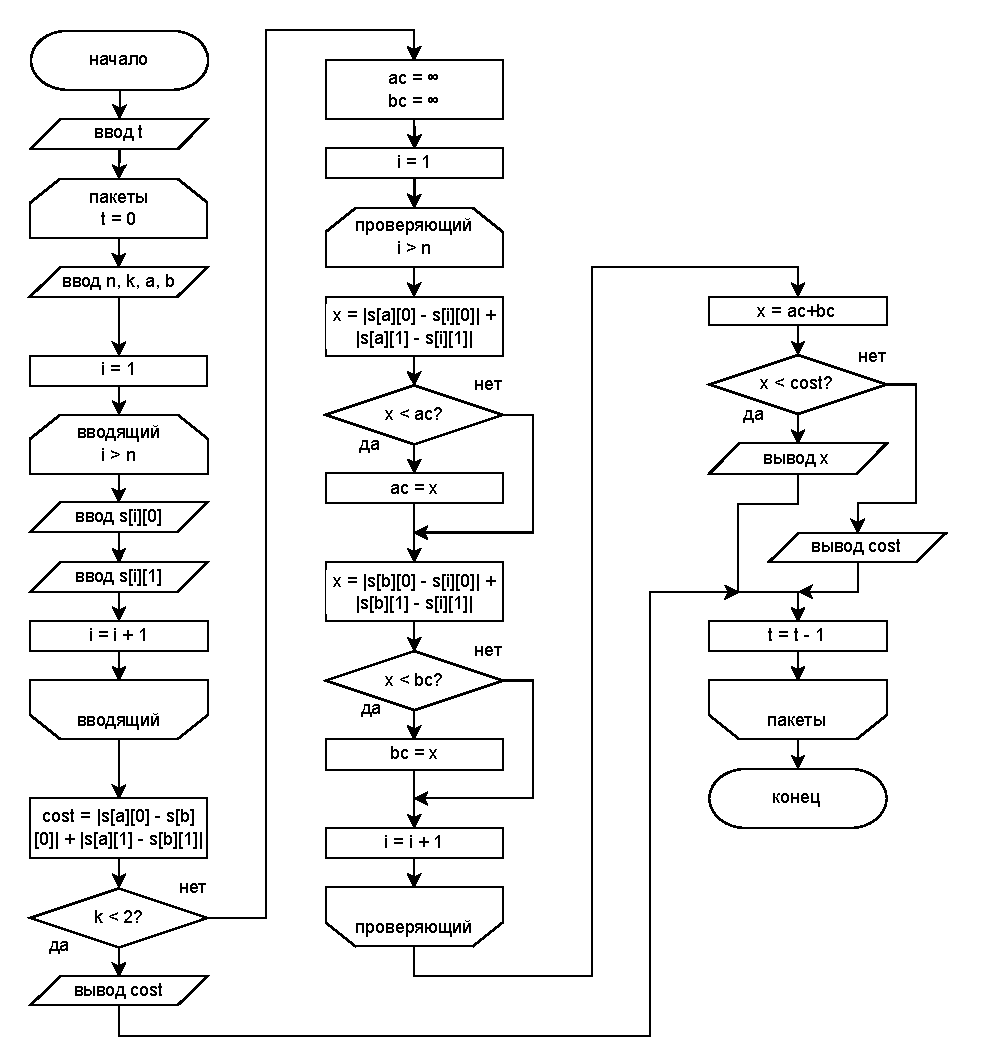
\includegraphics[width=17cm, keepaspectratio]{z1.pdf}
		\caption{Схема алгоритма задачи}
	\end{figure}
	\newpage
	\lstinputlisting[caption={Исходный код программы (C)}]{z1.c}
	\noindent
	Ссылка на успешное отправление: \\
	\indent
	https://codeforces.com/contest/1869/submission/371533360 \\
	\newline
	\noindent
	\textbf{Задание 520B:} \\
	\indent
	Цель задания -- узнать сколько раз нужно нажать кнопки чтобы прийти из числа N в число M имея операции: <<умножение на 2>> и <<вычитание 1>>. \\
	\newline
	Ссылка на задание: \\
	\indent
	https://codeforces.com/contest/520/problem/B \\
	\newline
	\noindent
	Для данного задания оптимальный алгоритм: \\
	\noindent
	Пока M > N: \\
	\indent
	Если M чётное: поделить M на 2 \\
	\indent
	Если M нечётное: вычесть 1 из M \\
	\indent 
	Счётчик увеличить на 1. \\
	\noindent
	Когда M <= N: \\
	\indent
	Вывести разницу (N - M) + счётчик. \\
	\newpage
	\begin{figure}[H]
		\centering
		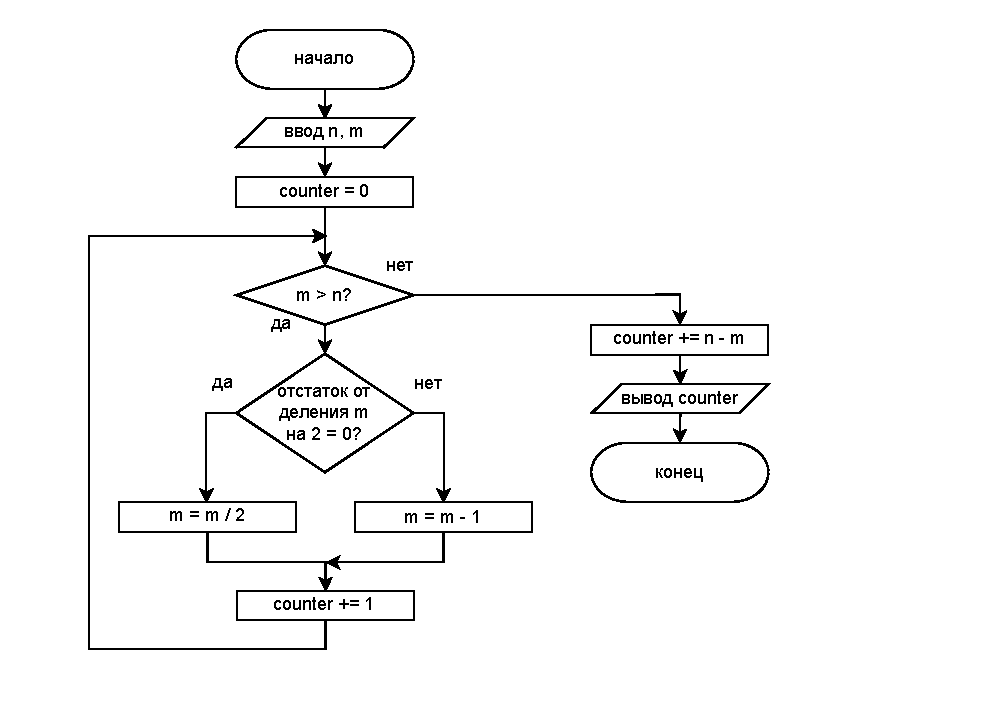
\includegraphics[width=17cm, keepaspectratio]{z2.pdf}
		\caption{Схема алгоритма задачи}
	\end{figure}
	\lstinputlisting[caption={Исходный код программы (C)}]{z2.c}
	\noindent
	Ссылка на успешное отправление: \\
	\indent
	https://codeforces.com/contest/520/submission/371758129 \\
	\newline
	\noindent
	\textbf{Задание 932B:} \\
	\indent
	Суть задачи: для каждого числа от 1 до 1 млн вычисляется цифровой корень g(x),
	сводящий число к однозначному путём многократного перемножения его ненулевых цифр.
	В ответе нужно для каждого из Q запросов посчитать,
	сколько чисел на отрезке $[l,\ r]$ имеют заданное значение $g(x)=k,\ (1 \leq k \leq 9)$. \\
	\newline
	Ссылка на задание: \\
	\indent
	https://codeforces.com/contest/932/problem/B \\

	Для решения задачи нужно предварительно вычислить для каждого числа от 1 до максимальной границы его однозначный корень,
	получаемый многократным перемножением ненулевых цифр.
	Затем для каждого из девяти возможных корней строится массив префиксных сумм,
	где элемент с индексом i хранит количество чисел от 1 до i с данным корнем.
	После этого каждый запрос на отрезке обрабатывается за O(1) вычитанием префиксных значений:
	результат для границы R минус результат для L-1.
	\newpage
	\begin{figure}[H]
		\centering
		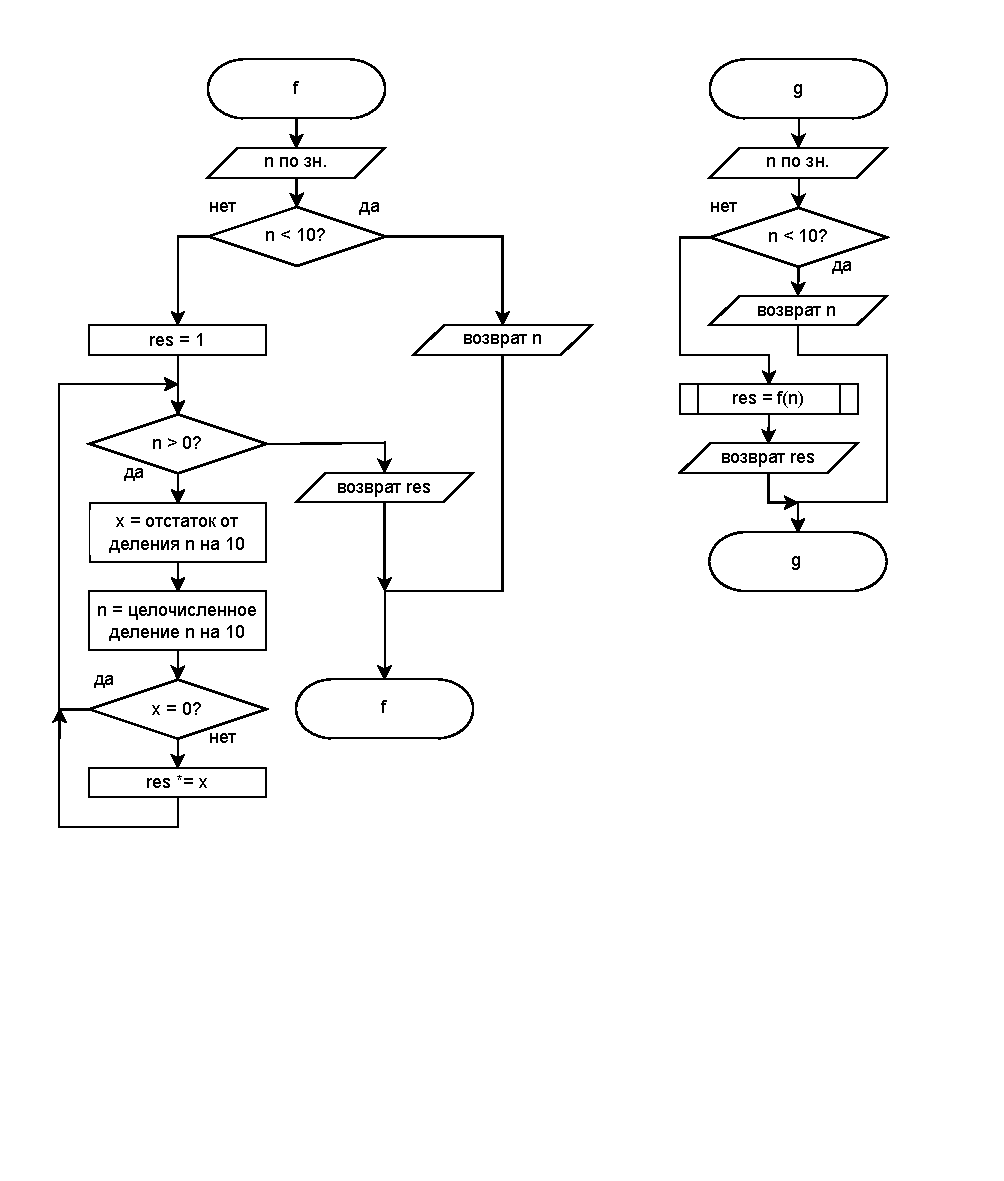
\includegraphics[width=17cm, keepaspectratio]{z3-1.pdf}
		\caption{Схема алгоритма задачи ч.1}
	\end{figure}
	\newpage
	\begin{figure}[H]
		\centering
		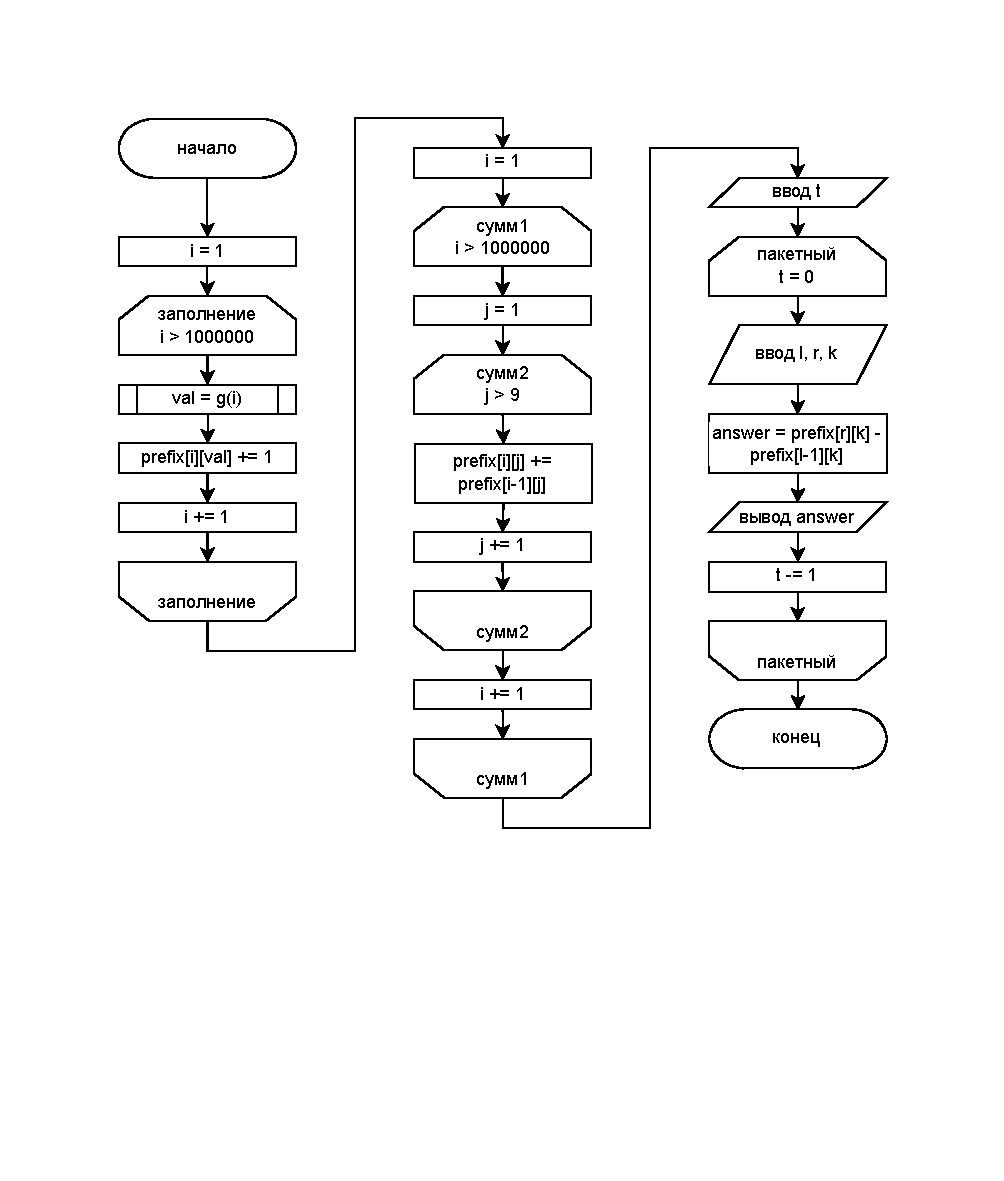
\includegraphics[width=17cm, keepaspectratio]{z3-2.pdf}
		\caption{Схема алгоритма задачи ч.2}
	\end{figure}
	\newpage
	\lstinputlisting[caption={Исходный код программы (C)}]{z3.c}
	\noindent
	Ссылка на успешное отправление: \\
	\indent
	https://codeforces.com/contest/932/submission/371785070 \\
	\newline
	\noindent
	\textbf{Задание 107A:} \\
	\indent
	В ориентированном графе, где у каждой вершины не более одного входящего и одного исходящего ребра,
	нужно найти все пути от источника (вершины с исходящим ребром, но без входящего)
	до стока (вершины с входящим ребром, но без исходящего) и для каждого такого пути
	определить минимальную пропускную способность (диаметр) на его рёбрах. \\
	\newline
	Ссылка на задание: \\
	\indent
	https://codeforces.com/contest/107/problem/A \\
	\newline
	\indent
	В данном решении находятся все цепи от источников (вершин без входящих рёбер, но с исходящим)
	до стоков (вершин без исходящих) в графе, где каждая вершина имеет не более одного входящего
	и одного исходящего ребра. Для каждой цепи вычисляется минимальная пропускная способность среди её рёбер,
	после чего выводится количество таких цепей, а для каждой — номер источника, номер стока и найденный минимум.
	\newpage
	\begin{figure}[H]
		\centering
		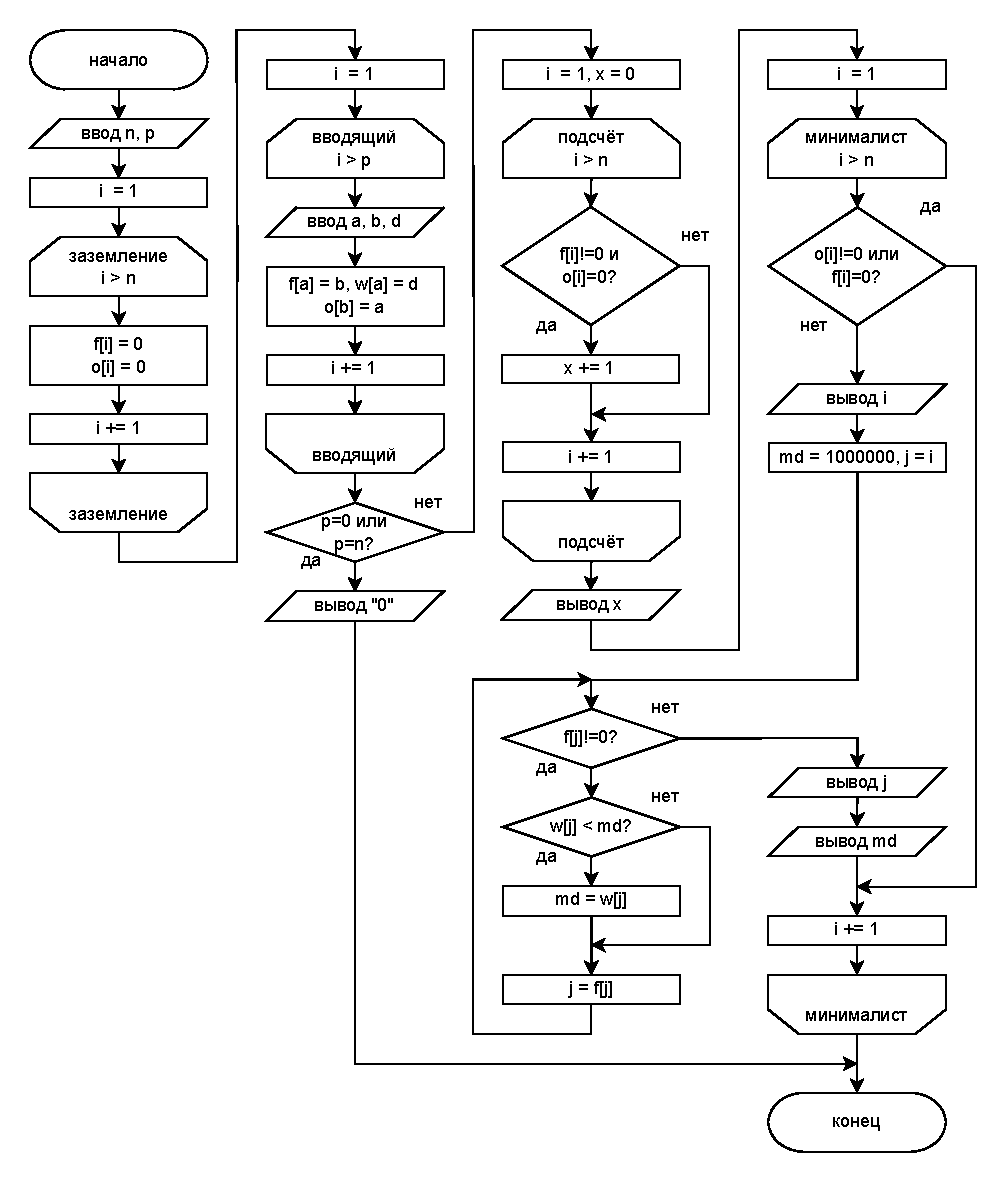
\includegraphics[width=17cm, keepaspectratio]{z4.pdf}
		\caption{Схема алгоритма задачи}
	\end{figure}
	\newpage
	\lstinputlisting[caption={Исходный код программы (C)}]{z4.c}

	\section*{Выводы}
	\noindent
	\indent В ходе выполнения лабораторной работы я научился применять несколько ключевых приёмов оптимизации, которые позволяют заменить прямое (часто переборное) решение на более эффективное. \\
	\indent Во-первых, использование жадного подхода вместо полного перебора вариантов. Например, в задаче с перелётами мы не перебираем все пары крупных городов, а ищем только ближайшие к пунктам А и В — это сокращает сложность с O(k²) до O(k). А в задаче с кнопками движение «от цели к исходному числу» оказалось проще и быстрее, чем прямой BFS. \\
	\indent Во-вторых, предварительная обработка данных (preprocessing) и префиксные суммы. Для задачи с цифровыми корнями мы один раз вычислили ответ для всех чисел до миллиона и построили префиксные массивы по каждому корню. Благодаря этому каждый запрос обрабатывается за O(1) вместо того, чтобы каждый раз заново считать корни на отрезке. \\
	\indent В-третьих, учёт структуры графа (не более одного входящего и одного исходящего ребра) позволил отказаться от сложных обходов вроде DFS — достаточно было пройти по цепочкам от источников к стокам, что дало линейную сложность. \\
	\indent Итог: главное, что я вынес — перед тем как писать «лобовое» решение, стоит проанализировать ограничения и найти закономерности. Жадность, предподсчёт, префиксные суммы и правильное использование условий задачи могут ускорить программу в сотни раз и уложиться в лимиты времени. \\
	
\end{document}
